\documentclass[10pt,a4paper]{article}
\usepackage[utf8]{inputenc}
\usepackage[magyar]{babel}
%\usepackage{t1enc}
\usepackage{fancyhdr}
\usepackage{amsmath}
\usepackage{amsfonts}
\usepackage{enumitem}
\usepackage{amssymb}
\usepackage{tikz}
\usepackage{float}
\usepackage{fancyvrb}

\usepackage[left=2cm,right=2cm,top=3cm,bottom=3cm]{geometry}
\usetikzlibrary{patterns}
\author{Török János}
\title{Vizsgafeladatok otthoni megoldásra}
\newfloat{Diagram}{htbp}{dia}

%\usepackage[framemethod=tikz]{mdframed}
%\usepackage{lipsum}
%\definecolor{mycolor}{rgb}{0.122, 0.435, 0.698}
%\newmdenv[innerlinewidth=0.5pt, roundcorner=4pt,linecolor=mycolor,innerleftmargin=6pt,
%innerrightmargin=6pt,innertopmargin=6pt,innerbottommargin=6pt]{mybox}



\begin{document}
\maketitle
\pagestyle{fancy}
\lhead{Török János}
\rhead{Piacszerkezetek beadandó}

\section{Feladat}
Egy távoli vidéken lévő szénbányában 10 \$/GJ határköltséggel termelnek feketeszenet. A bányához közeli településen élő háztartások téli tüzelőanyag iránti éves kereslete (együttesen) D(p)=100-2p. A mennyiségeket GJ-ban mérjük.

\begin{enumerate}[label=(\alph*)]
\item A településen a helyi kitermelésű szén az egyetlen szóba jöhető téli tüzelőanyag. Milyen szénárat szabjon a bánya, hogy a lehető legmagasabb nyereséget érje el? Mennyi szenet tüzelnek el a háztartások összesen ezen az áron?

\begin{Diagram}
\centering
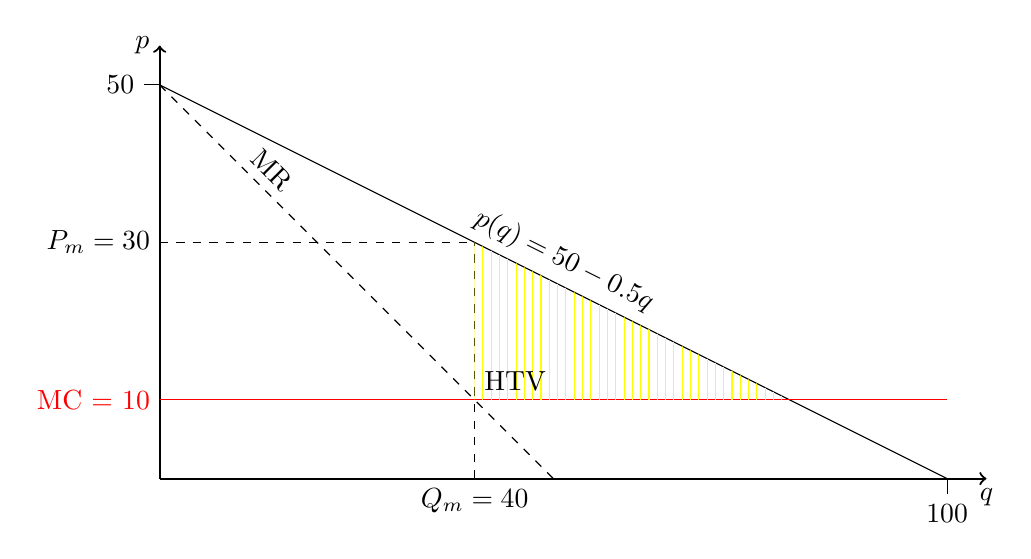
\begin{tikzpicture}[scale = .1]
\usetikzlibrary{calc}
% draw grid lines
%	\draw[very thin, color=lightgray!50, step=10] (0, 0) grid (104, 54);
	\draw[thick, ->] (0,0) -- (105, 0)  node[below] {$q$};
	\draw[thick, ->] (0,0) -- (0, 55) node[left] {$p$};
	
	\draw[] (0,50) -- (100, 0) node [midway, above, sloped] {$p(q) = 50-0.5q$};
	\draw[dashed] (0,50) -- (50, 0) node [near start, above, sloped] {MR};
	\draw[] (0,50) -- (-2, 50) node [left] {50};
	\draw[] (100,0) -- (100, -2) node [below] {100};
	\draw[color=red,] (0,10) node [left] {MC = 10}-- (100, 10) ;
		
	\draw[dashed] (40,0) node[below]{$Q_m = 40$}-- (40, 30);
	\draw[dashed] (0,30) node[left]{$P_m = 30$}-- (40, 30);
% area color
	\path[pattern= vertical lines, pattern color=yellow](40,10) 
		node [above right]{HTV}--(40,30)--(80,10);
\end{tikzpicture}
\end{Diagram}


$MC = 10 \$/GJ$  

$D(p) = 100-2p \rightarrow	p = 50-\displaystyle\frac{1}{2}q. $

$\pi = TR -TC = p\cdot q - MC \cdot q = (50-q/2) \cdot q - MC \cdot q $

A monopolium Q megválasztásán keresztül kíván profitot maximalizálni:

$\max\limits_{q} \pi  = (50-q/2) \cdot q - MC \cdot q $ 
határprofitját nullával teszi egyenlővé, ez az elsőrendű feltétel:

$\displaystyle\frac{d\pi}{dq} = MR-MC$

$(-\displaystyle\frac{1}{2}Q^2 + 50Q)' = -Q +50 = 10$

$Q_m = 40 \rightarrow P_m = 30 $

A háztartások 40 GJ szenet tüzelnek el 30 \$/GJ áron.




\item Mi lesz a Lerner-index értéke a profitmaximalizáló pontban?

$LI = \displaystyle\frac{P-MC}{P} =\frac{30-10}{30} = 66,67 \%$

A piaci erő mérésére alkalmazott Lerner-index az ár és a határköltség különbségének az árhoz viszonyított arányával, azaz a relatív árréssel azt mutatja hogy a vállalat mennyire képes terméke árát a rövid távú határköltsége fölé emelni. Versenyzői piacon P=MC lenne. A Lerner index azt is kifejezi, hogy mennyire rugalmas a kereslet ( $LI = -\displaystyle\frac{1}{\epsilon}$). Monopóliumnál minél kevésbé rugalmasabb a kereslet az ár annál messzebb esik a határköltségtől. Ebben az esetben $\epsilon = -1.5$ Azaz a piaci erő egyben fordítottan arányos a vállalattal szemben állított kereslet rugalmasságával.

\item Mekkora holtteherveszteséggel jár a monopólium működése?

Versenyzői mennyiség\footnote{$(a-c)/b = (50-10)/0.5 = 80$}
$-\displaystyle\frac{1}{2}Q_c +50 = 10 \rightarrow Q_c = 80$



$HTV = \displaystyle\frac{(Q_c - Q_m) \cdot (P_m-MC)}{2} = (80-40) \cdot (30-10) /2 = 400 $


\item Egy szénkereskedelmi vállalkozás a szénbányához képest jóval magasabb költséggel (25 \$/GJ) lenne képes szenet szállítani egy másik megyéből, amennyiben pozitív profitlehetőséget látna. Hogyan befolyásolja a szénkereskedő feltűnése a szénbánya árazási stratégiáját, ha tudatában van annak, hogy a kereskedő a szénbánya árának megismerését követően határoz a belépésről és az alkalmazott árakról? Mi lesz a piaci egyensúly, melyik vállalkozás mennyi szenet fog értékesíteni a településen?

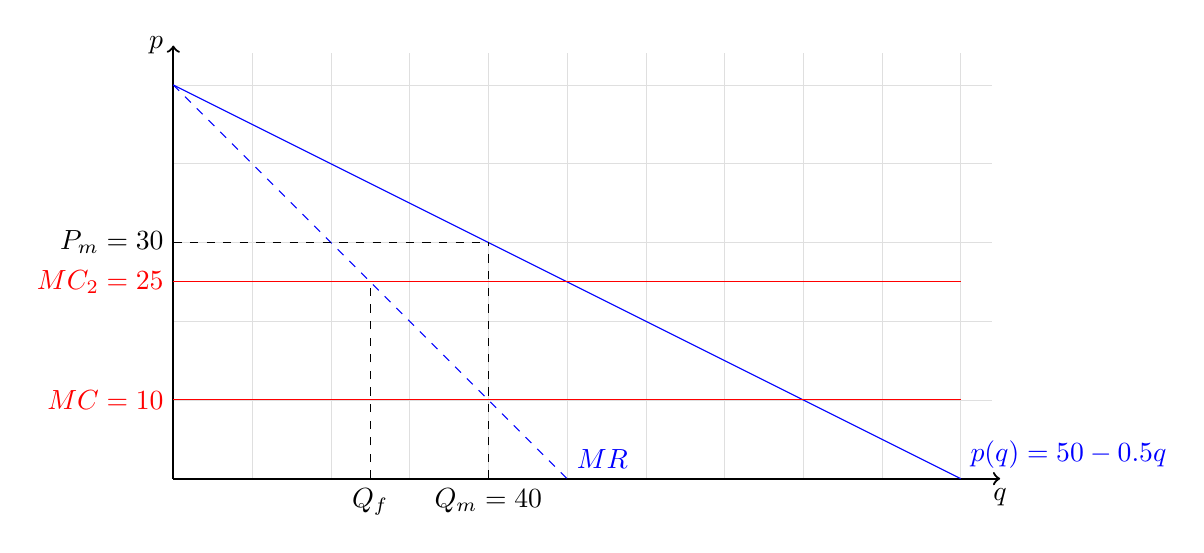
\begin{tikzpicture}[scale = .1]
\usetikzlibrary{calc}
% draw grid lines
	\draw[very thin, color=lightgray!50, step=10] (0, 0) grid (104, 54);
	
% draw Coordinates
	\draw[thick, ->] (0,0) -- (105, 0)  node[below] {$q$};
	\draw[thick, ->] (0,0) -- (0, 55) node[left] {$p$};

% plot line y = 4-x
	\draw[color=blue, domain=0:100] plot (\x,{50-0.5*\x}) 
		node[above right] {$p(q) = 50-0.5q$};	
	\draw[color=blue, dashed, domain=0:50] plot (\x,{50-1*\x}) 
		node[above right] {$MR$};		

	\draw[color=red] (0,10) node[left]{$MC = 10$}-- (100, 10);
	\draw[color=red] (0,25) node[left]{$MC_2 = 25$}-- (100, 25);
		
	\draw[dashed] (40,0) node[below]{$Q_m = 40$}-- (40, 30);
	\draw[dashed] (0,30) node[left]{$P_m = 30$}-- (40, 30);
	\draw[dashed] (25,0) node[below]{$Q_f$}-- (25, 25);
\end{tikzpicture}

Stratégia befolyásolása: 

 
Az $p<25$ alatt az új vállalkozás már nem termel. Pusztán a belépése korlátozni tudja a domináns vállalat piaci erőfölényét. $p>25$ feletti ár esetén az új belépő egészen $Q_f$ mennyiségig  növelheti a termelését ezzel a domináns vállalat profittól esik el.
A domináns stratégiája során nem csökkentheti a mennyiséget ($Q_m$) hiszen akkor még magasabb ár alakulna ki ami új belépőket  vonzana.
Míg monopóliumnál csak a keresleti görbét és a hozzá tartozó $MR$ határbevételi görbét kellett figyelni ebben a szituációban  már az optimális ár megválasztásával az új belépő lehetséges viselkedését is figyelni kell.

Itt nincs információnk arról, hogy a belépésnek korlátai lennének. Ezért 25 feletti árnál várható,  hogy akár újabb vállalatok is belépnek, hiszen pozitív profitra tehetnek szert (MC = 25-t feltételezve a szegélynek).
Tehát a szénbánya két lehetőség közül választhat:
\begin{enumerate}[label=(\roman*)]

\item úgy játszik, hogy 25 feletti árat mutat az új potenciális belépőnek (azaz a $P_m=30$ árat), ekkor az be fog lépni ezzel a szénbánya profittól esik el; további belépőkre lehet ekkor számítani ami azt eredményezi hogy a szegély versenyzőként fog működni és p= 25-ig az ahhoz tartozó keresletet ki fogja elégíteni.


\item ha p = 25 árat mutat az új belépőnek, ezzel megerősíti őt abban hogy ezen a piacon nincs új belépő számára pozitív profitlehetőség.  Ha ezt az árat tartja is akkor (A) terület profitjától elesik és (C) terület többlet költséggel szembesül azzal hogy a kereslete $Q=50$ ig felmegy, és mindezt (B) területnyi többletbevétellel tudja csak kompenzálni.

Ha az új vállalkozás eláll a belépéstől akkor a mennyiséget ujra visszacsökkentheti 40-ig és visszaáll a monopol piaci egyensúly.


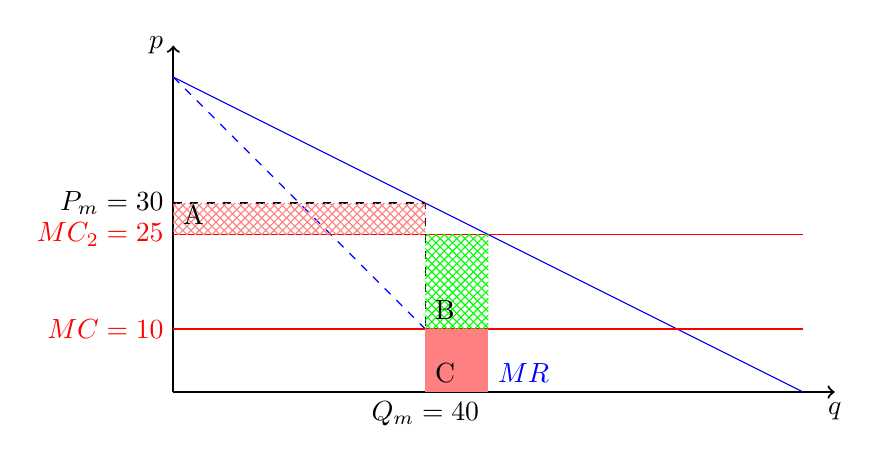
\begin{tikzpicture}[scale = .08]

% draw grid lines
	%\draw[very thin, color=lightgray!50, step=10] (0, 0) grid (104, 54);
	
% draw Coordinates
	\draw[thick, ->] (0,0) -- (105, 0)  node[below] {$q$};
	\draw[thick, ->] (0,0) -- (0, 55) node[left] {$p$};

% plot line y = 4-x
	\draw[color=blue, domain=0:100] plot (\x,{50-0.5*\x});	
	\draw[color=blue, dashed, domain=0:50] plot (\x,{50-1*\x}) 
		node[above right] {$MR$};		

	\draw[color=red] (0,10) node[left]{$MC = 10$}-- (100, 10);
	\draw[color=red] (0,25) node[left]{$MC_2 = 25$}-- (100, 25);
		
	\draw[dashed] (40,0) node[below]{$Q_m = 40$}-- (40, 30);
	\draw[dashed] (0,30) node[left]{$P_m = 30$}-- (40, 30);
	
% area color
	\path[pattern= crosshatch, pattern color=red!50] 
	(0,25) node [above right]{A}--(0,30)--(40,30)--(40,25);

	\path[pattern= crosshatch, pattern color=green] 
	(40,10) node [above right]{B}--(40,25)--(50,25)--(50,10);
	
	\path[fill, color=red!50] 
	(40,0) node [above right, color=black]{C}--(40,10)--(50,10)--(50,0);

\end{tikzpicture}

Ezt a (ii) helyzetet ragadozó magatartásnak is felfoghatjuk\footnote{Evans-Schmalensee  azokat a cselekvéseket nevezi ragadozónak, amely csak akkor racionálisak, ha megszüntetik vagy gyengítik a versenyt} itt tudatosan feláldozásra kerül a profit egy része az erőfölény megtartásáért \footnote{pl: Empire Gas Corporation 1970: belépési korlátok szintén hiányoztak,  kényszerítette versenytársait hogy piacról kilépjenek vagy hasonló magas árat alkalmazzanak, összességében veszteséges stratégia volt.}. A szabályozó közbeavatkozására van szükség.
\end{enumerate}


\item Az a-c) feladatban leírt helyzetben a település polgármestere (aki természetesen a lakosok érdekeit képviseli) tárgyalásokat kezdeményez a szénbánya tulajdonosával. Azt szeretné elérni, hogy egy éves fix "iparűzési támogatásért" cserébe a bánya 20 \$/GJ-ra szállítsa le a szén árát. A támogatás összegét természetesen a háztartásoknak kell összedobni egyenlő arányban. 

Legalább mennyi pénzt kell a bányának átutalni ahhoz, hogy belemenjen egy ilyen alkuba? 



Itt is többféle eset történhet meg:

- ha a vállalat leszállítja az árat, de nem változtat a kibocsátás mennyiségén: ekkor rövid távon  elég ha a kiesett profitot kéri iparűzési támogatásért, viszont ekkor hiány lesz a piacon, egyensúlytalanság, a jólét nem változna,  ráadásul várhatóan új vállalatok lépnének be akik kitöltenék a hiányt de 20 feletti $MC$ esetén kérnék az önkormányzat támogatását. 

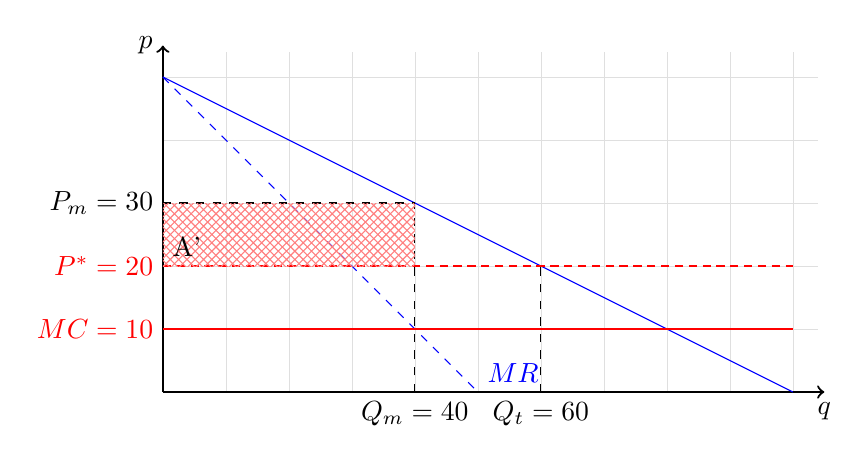
\begin{tikzpicture}[scale = .08]

% draw grid lines
	\draw[very thin, color=lightgray!50, step=10] (0, 0) grid (104, 54);
	
% draw Coordinates
	\draw[thick, ->] (0,0) -- (105, 0)  node[below] {$q$};
	\draw[thick, ->] (0,0) -- (0, 55) node[left] {$p$};

% plot line y = 4-x
	\draw[color=blue, domain=0:100] plot (\x,{50-0.5*\x});	
	\draw[color=blue, dashed, domain=0:50] plot (\x,{50-1*\x}) 
		node[above right] {$MR$};		

	\draw[color=red] (0,10) node[left]{$MC = 10$}-- (100, 10);
	\draw[densely dashed, color=red] (0,20) node[left]{$P^* = 20$}-- (100, 20);
		
	\draw[dashed] (0,30) node[left]{$P_m = 30$}-- (40, 30);
	
	\draw[dashed] (40,0) node[below]{$Q_m = 40$}-- (40, 30);
	\draw[dashed] (60,0) node[below]{$Q_t = 60$}-- (60, 20);
	
% area color
	\path[pattern= crosshatch, pattern color=red!50] 
	(0,20) node [above right]{A'}--(0,30)--(40,30)--(40,20);

\end{tikzpicture}

$Q(P=20) = 100-2P$

$Q(P=20) = 100-40$

$Q(P=20) = 60$

Elveszett árrés ($A'$): $(30-20) \cdot 40 = 400$

- ha a vállalat leszállítja az árat P=20-ra akkor azon a szinten Q = 60 a piaci igény, monopoliumunknak azonban Q=30 lenne az optimális.

ebben az esetben a monopolium: 

elveszti az A' területnyi profitot: ($A'$): $(30-20) \cdot 40 = -400$ 

új  forgalmat realizál ($B'$): $(60-40) \cdot (20-10) = +200$

extra költségek is megjelennek ($C'$): $(60-40) \cdot 10 = -200$ 

feltéve hogy nincs kapacitáskorlátja ( ha lenne akkor  azt is megkérné támogatásként hogy bővítsen). Ez összesen 400\$

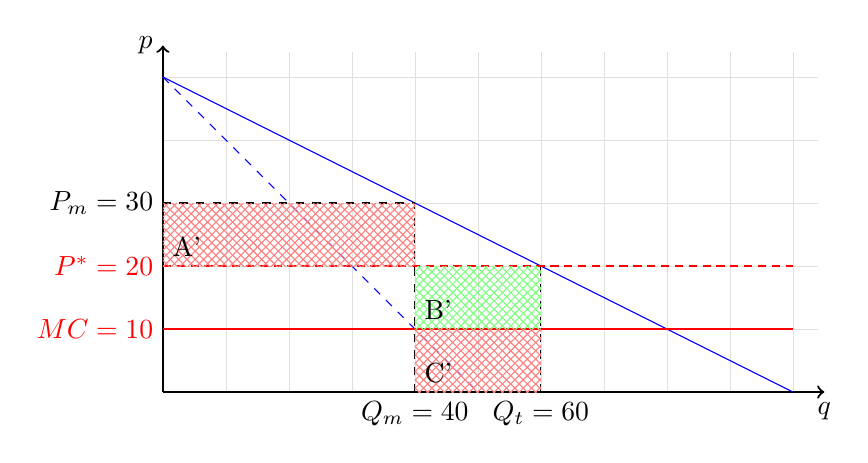
\begin{tikzpicture}[scale = .08]
% draw grid lines
	\draw[very thin, color=lightgray!50, step=10] (0, 0) grid (104, 54);
	
% draw Coordinates
	\draw[thick, ->] (0,0) -- (105, 0)  node[below] {$q$};
	\draw[thick, ->] (0,0) -- (0, 55) node[left] {$p$};

% plot line y = 4-x
	\draw[color=blue, domain=0:100] plot (\x,{50-0.5*\x});	
	\draw[color=blue, dashed, domain=0:50] plot (\x,{50-1*\x});		

	\draw[color=red] (0,10) node[left]{$MC = 10$}-- (100, 10);
	\draw[densely dashed, color=red] (0,20) node[left]{$P^* = 20$}-- (100, 20);
		
	\draw[dashed] (0,30) node[left]{$P_m = 30$}-- (40, 30);
	
	\draw[dashed] (40,0) node[below]{$Q_m = 40$}-- (40, 30);
	\draw[dashed] (60,0) node[below]{$Q_t = 60$}-- (60, 20);
	
% area color
	\path[pattern= crosshatch, pattern color=red!50] 
	(0,20) node [above right]{A'}--(0,30)--(40,30)--(40,20);
	
	\path[pattern= crosshatch, pattern color=green!50] 
	(40,10) node [above right]{B'}--(40,20)--(60,20)--(60,10);
	
	\path[pattern= crosshatch, pattern color=red!50] 
	(40,0) node [above right]{C'}--(40,10)--(60,10)--(60,00);

\end{tikzpicture}

\textbf{Legfeljebb mennyi pénzt hajlandó a város összedobni erre a célra?}
A támogatással nyerhető fogyasztói többletnek megfelelő összeget:

$\Delta FT= (30-20) \cdot 40 + \displaystyle\frac{(60-40) \cdot (30-10)}{2}$

$\underline{\Delta FT= 500}$  Tehát a város maximum 500-t hajlandó erre a célra összedobni.

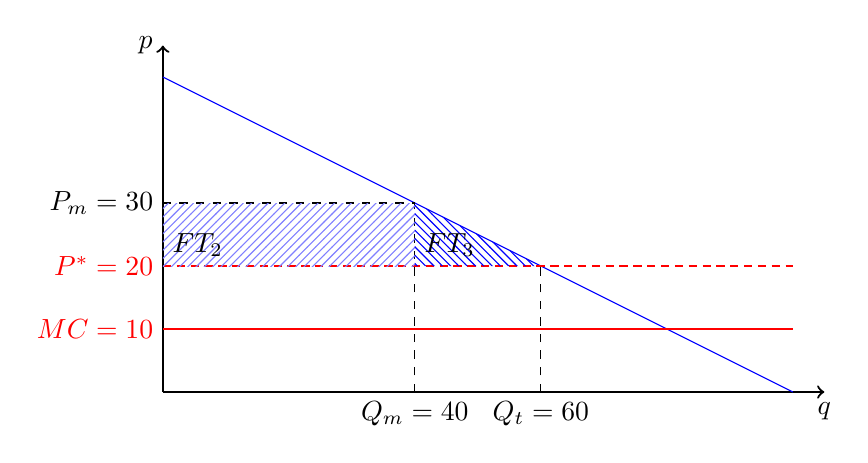
\begin{tikzpicture}[scale = .08]
% draw Coordinates
	\draw[thick, ->] (0,0) -- (105, 0)  node[below] {$q$};
	\draw[thick, ->] (0,0) -- (0, 55) node[left] {$p$};

% plot line y = 4-x
	\draw[color=blue, domain=0:100] plot (\x,{50-0.5*\x});	
	\draw[color=red] (0,10) node[left]{$MC = 10$}-- (100, 10);
	\draw[densely dashed, color=red] (0,20) node[left]{$P^* = 20$}-- (100, 20);
		
	\draw[dashed] (0,30) node[left]{$P_m = 30$}-- (40, 30);
	
	\draw[dashed] (40,0) node[below]{$Q_m = 40$}-- (40, 30);
	\draw[dashed] (60,0) node[below]{$Q_t = 60$}-- (60, 20);
	
% area color
	
	\path[pattern= north east lines, pattern color=blue!50] 
	(0,20) node [above right]{$FT_2$}--(0,30)--(40,30)--(40,20);

	\path[pattern= north west lines, pattern color=blue] 
	(40,20) node [above right]{$FT_3$}--(40,30)--(60,20);
	
\end{tikzpicture}
 
 
Ezek alapján van-e kilátás arra, hogy a megállapodást meg fogják kötni?

Igen. Az elérhető fogyasztói többlet növekmény nagyobb mint a monopoliumnak adandó iparűzési támogatás mint költség.
\end{enumerate}
 
 

\section{Feladat}

Egy távoli országban két nagykereskedő (X és Y) értékesít villamos energiát a kiskereskedőknek, akinek az együttes kereslete a Q=200-p függvénnyel írható le, ahol Q a keresett mennyiség TWh-ban, p pedig az ár millió \$-ban kifejezve. Mindkét nagykereskedő 20 millió \$/TWh határköltséggel tudja biztosítani a villamos energiát. 
\begin{enumerate}[label=(\alph*)]

\item A két nagykereskedő árverésen értékesíti a villamos energiát, melynek során az árverésre bocsátott mennyiséget határozzák meg, az ár kialakítását pedig a piacra bízzák. Mi lesz a piaci egyensúly (értékesített mennyiség, árak, profitok), amennyiben mindkét vállalat azt feltételezi versenytársáról, hogy az tőle függetlenül (és vele egy időben) dönt az értékesített mennyiségről?

\begin{align}
MC &= 20 	\nonumber\\
Q &= 200-P 	 \hspace{1cm}\rightarrow P = 200-Q \nonumber\\
Q &= q_1+q_2	\hspace{1cm}\rightarrow P = 200-q_1-q_2 \nonumber\\
\nonumber\\
\pi &= TR - TC \nonumber\\
TR &= p \cdot  q \nonumber\\
\pi &= pq_1-C(q_1)\nonumber\\
\pi &= (200-q_1-q_2)q_1-C(q_1) \\
\pi &= 200q_1-q_1^2-q_1q_2-C(q_1) \nonumber\\
MR &= \frac{\partial TR}{\partial q_1} \nonumber\\
MR &= 200-2q_1-q_2 \nonumber\\
MR-MC &= 0  \hspace{2cm} /ERF\\
(200-2q_1-q_2)-20 &=0 \nonumber\\
180-2q_1-q_2 &= 0 \nonumber\\
180-q_2 &= 2q_1 \nonumber\\
Reakci\acute{o}f\ddot{u}ggv\acute{e}nyek:\hspace{2cm} \displaystyle\frac{180-q_2}{2} &= q_1 \hspace{2cm}\rightarrow  q_2=\displaystyle\frac{180-q_1}{2} 
\\
\frac{180-\frac{180-q_1}{2}}{2} &= q_1  \nonumber\\
q_1 &= 60 \hspace{2cm} q_2=60 \\
P &= 200-60-60 = 80 
\end{align}

A profitfüggvénybe  behelyettesítve (1) az átalakított inverz keresleti függvényt majd az elsőrendű feltételt alkalmazza és parciálisan $q_1$ szerint lederiválva 0-ra rendezve a két reakciófüggvény(3) került kifejezésre.

Ezen reakciófüggvények megoldásából (4) megkapjuk az X vállalat $q_1$ és a Y vállalat által termelt $q_2$ mennyiséget. Ezen $q_1+q_2$ mennyiségekhez tartozó piaci egyensúlyi ár 80 millió \$/TWh.

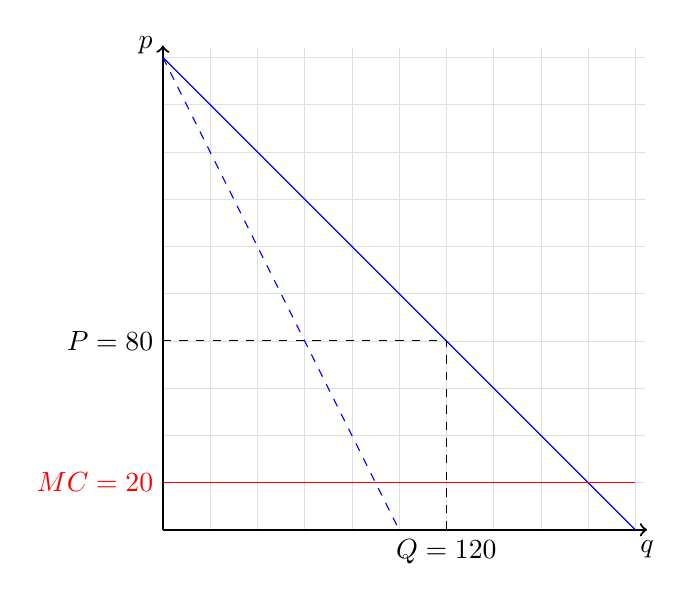
\begin{tikzpicture}[scale = .03]
% draw grid lines
	\draw[very thin, color=lightgray!50, step=20] (0, 0) grid (204, 204);	
% draw Coordinates
	\draw[thick, ->] (0,0) -- (205, 0)  node[below] {$q$};
	\draw[thick, ->] (0,0) -- (0, 205) node[left] {$p$};
% plot line y = 4-x
	\draw[color=blue, domain=0:200] plot (\x,{200-1*\x});	
	\draw[color=blue, dashed, domain=0:100] plot (\x,{200-2*\x});	
	\draw[color=red] (0,20) node[left]{$MC = 20$}-- (200, 20);	
	\draw[dashed] (120,0) node[below]{$Q = 120$}-- (120, 80);
	\draw[dashed] (0,80) node[left]{$P = 80$}-- (120, 80);	
\end{tikzpicture}

A grafikus megoldásból látható hogy a Cournot duopolium egyensúlyi mennyisége a monopol mennyiség(MC=MR) és a versenyzői mennyiség (p=MC) közé esik.

Az elérhető profit egyenként:

$\pi=TR-TC = P \cdot q1 - P \cdot MC = 80 \cdot 60 - 60 \cdot 20 = \underline{3600}$ (millió \$)

\item A nagykereskedők egy iparági konferencián megegyeznek, hogy összehangolják az árverésre bocsátott mennyiségeiket annak érdekében, hogy magasabb profitot érjenek el.
Mekkora egyenként értékesítendő mennyiségeket fognak közösen meghatározni a vállalkozások, és milyen profitot érhetnek el ezzel (egyenként)?

Az így kialakuló vállalatszövetség egy kartell, amely egy kooperatív oligopolista piacszerkezet. Ennek a piacszerkezetnek a célja, hogy a vállalatok együttes profitját maximalizálja. 

$\max\limits_{q_1, q_2} \{p(q_1+q_2)[q_1+q_2] -c_1(q_1) -c_2(q_2)\}$

A monopolegyenletet kell megoldani és az abból megkapott mennyiséget lesz a kartell összkibocsátása.
\begin{align}
TR &= P*Q \nonumber\\
TR &= (200-Q)*Q \nonumber\\
TR &= 200Q-Q^2 \nonumber\\
MR &= 200-2Q \nonumber\\
ERF: MR-MC &= 0 \nonumber\\
200-2Q -20 &= 0 \nonumber\\
Q &= 90 \nonumber\\
q_1 &= 45 \hspace{1cm} q_2 = 45 \nonumber\\
P &= 200-q_1-q_2 \nonumber\\
P &= 110  \nonumber
\end{align}

Az elérhető profit egyenként:

$\pi=TR-TC = P \cdot q1 - P \cdot MC = 110 \cdot 45 - 45 \cdot 20 = \underline{4050}$ (millió \$)

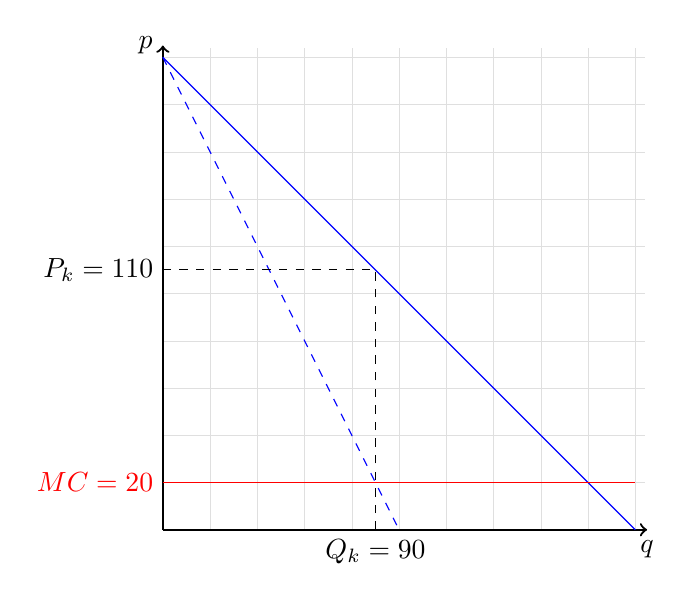
\begin{tikzpicture}[scale = .03]
% draw grid lines
	\draw[very thin, color=lightgray!50, step=20] (0, 0) grid (204, 204);	
% draw Coordinates
	\draw[thick, ->] (0,0) -- (205, 0)  node[below] {$q$};
	\draw[thick, ->] (0,0) -- (0, 205) node[left] {$p$};
	
% plot line y = 4-x
	\draw[color=blue, domain=0:200] plot (\x,{200-1*\x});	
	\draw[color=blue, dashed, domain=0:100] plot (\x,{200-2*\x});	
	\draw[color=red] (0,20) node[left]{$MC = 20$}-- (200, 20);	
	\draw[dashed] (90,0) node[below]{$Q_k = 90$}-- (90, 110);
	\draw[dashed] (0,110) node[left]{$P_k = 110$}-- (90, 110);	
\end{tikzpicture}

\item Az értékesítendő mennyiségről való megegyezést követően mindkét nagykereskedő még utoljára átgondolja (önállóan), hogy mi lenne számára az optimális stratégia. 
Mekkora mennyiség árverésére bocsátásával tudják maximalizálni profitjukat a nagykereskedők, ha azt feltételezik a másikról, hogy az betartja a megállapodást?

$q_1$ vállalat kibocsátása nem változik, továbbra is 45-t termel.

$q_2$ reakciófüggvénye ekkor: $q_2 = \displaystyle\frac{180-45}{2} = 67,5$

Ehhez tartozó ár: $P = 200-67.5 - 45 = 87.5$

$\pi_2= P \cdot q_2 - q_2 \cdot MC = 87.5 \cdot 67.5 - 67.5 \cdot 20 = 4556.25$

Hasonló az eredmény ha a keresleti függvényből levonjuk $q_1$ kibocsátását.

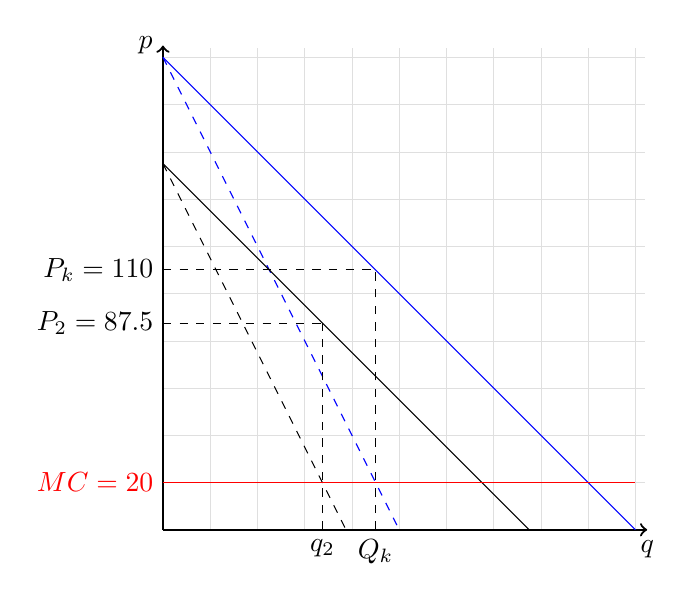
\begin{tikzpicture}[scale = .03]
% draw grid lines
	\draw[very thin, color=lightgray!50, step=20] (0, 0) grid (204, 204);	
% draw Coordinates
	\draw[thick, ->] (0,0) -- (205, 0)  node[below] {$q$};
	\draw[thick, ->] (0,0) -- (0, 205) node[left] {$p$};
% plot line 
	\draw[color=blue, domain=0:200] plot (\x,{200-1*\x});	
	\draw[color=blue, dashed, domain=0:100] plot (\x,{200-2*\x});
	
	\draw[domain=0:155] plot (\x,{155-\x});
	\draw[dashed, domain=0:77.5] plot (\x,{155-2*\x}) ;
% Pricelines
	\draw[color=red] (0,20) node[left]{$MC = 20$}-- (200, 20);	

	\draw[dashed] (90,0) node[below]{$Q_k$}-- (90, 110);
	\draw[dashed] (0,110) node[left]{$P_k = 110$}-- (90, 110);		

	\draw[dashed] (67.5,0) node[below]{$q_2$}-- (67.5, 87.5);
	\draw[dashed] (0, 87.5) node[left]{$P_2 = 87.5$}-- (67.5, 87.5);		
\end{tikzpicture}



Milyen árszint alakul ki az aukción, ha mindkét vállalkozás ezt a mennyiséget ajánlja fel?

Ha mindketten arra játszanak hogy a másik nem változtat, de ők igen, akkor mind a ketten a $q_{1/2} = \displaystyle\frac{180-45}{2} = 67,5$ reakciófüggvény szerinti mennyiséget termelik.

Így az összkibocsátás 2* 67,5 lesz = 135 lesz. Ehhez tartozó ár: $P = 200-2 \cdot 67.5 = 65$ 
A fogyasztók nyernek a kartell kudarcából: nagyobb mennyiség és így alacsonyabb ár alakul ki mint monopolárak esetén. a holt teher veszteség csökken.




\end{enumerate}
\end{document}
